\documentclass{beamer}

\mode<presentation> {
	% The Beamer class comes with a number of default slide themes
	% which change the colors and layouts of slides. Below this is a list
	% of all the themes, uncomment each in turn to see what they look like.
	
	%\usetheme{default}
	%\usetheme{AnnArbor}
	%\usetheme{Antibes}
	%\usetheme{Bergen}
	%\usetheme{Berkeley}
	%\usetheme{Berlin}
	%\usetheme{Boadilla}
	%\usetheme{CambridgeUS}
	%\usetheme{Copenhagen}
	%\usetheme{Darmstadt}
	%\usetheme{Dresden}
	%\usetheme{Frankfurt}
	%\usetheme{Goettingen}
	%\usetheme{Hannover}
	%\usetheme{Ilmenau}
	%\usetheme{JuanLesPins}
	%\usetheme{Luebeck}
	\usetheme{Madrid}
	%\usetheme{Malmoe}
	%\usetheme{Marburg}
	%\usetheme{Montpellier}
	%\usetheme{PaloAlto}
	%\usetheme{Pittsburgh}
	%\usetheme{Rochester}
	%\usetheme{Singapore}
	%\usetheme{Szeged}
	%\usetheme{Warsaw}
	
	% As well as themes, the Beamer class has a number of color themes
	% for any slide theme. Uncomment each of these in turn to see how it
	% changes the colors of your current slide theme.
	
	%\usecolortheme{albatross}
	\usecolortheme{beaver}
	%\usecolortheme{beetle}
	%\usecolortheme{crane}
	%\usecolortheme{dolphin}
	%\usecolortheme{dove}
	%\usecolortheme{fly}
	%\usecolortheme{lily}
	%\usecolortheme{orchid}
	%\usecolortheme{rose}
	%\usecolortheme{seagull}
	%\usecolortheme{seahorse}
	%\usecolortheme{whale}
	%\usecolortheme{wolverine}
	
	%\setbeamertemplate{footline} % To remove the footer line in all slides uncomment this line
	%\setbeamertemplate{footline}[page number] % To replace the footer line in all slides with a simple slide count uncomment this line
	
	%\setbeamertemplate{navigation symbols}{} % To remove the navigation symbols from the bottom of all slides uncomment this line
}
\usepackage[backend=biber]{biblatex}
\setbeamertemplate{caption}[numbered]
\setbeamertemplate{enumerate items}[default]
\newcommand{\btVFill}{\vskip0pt plus 1filll}
\usepackage{algorithm}
\usepackage{amsmath}
\usepackage{caption}
\usepackage{xcolor}
%----------------------------------------------------------------------------------------
%	TITLE PAGE
%----------------------------------------------------------------------------------------

\title[VRP Column Generation]{How to Implement Column Generation for Vehicle Routing}
\author{Sean Kelley} % Your name
\date{26 January 2023} % Date, can be changed to a custom date

\AtBeginSection[]{
	\begin{frame}
		\vfill
		\centering
		\begin{beamercolorbox}[sep=8pt,center,shadow=true,rounded=true]{title}
			\usebeamerfont{title}\insertsectionhead\par%
		\end{beamercolorbox}
		\vfill
	\end{frame}
}

\begin{document}
	
	\begin{frame}
		\titlepage % Print the title page as the first slide
	\end{frame}

	\begin{frame}{Overview}
		\tableofcontents
	\end{frame}

	\section{Why Implement Column Generation for Vehicle Routing}
	
	\begin{frame}[t]
		\frametitle{Context}
		\begin{itemize}
			\item Vehicle Routing Problems (VRPs) are hard to solve directly (e.g. as a mixed-integer program (MIP)).
			\item There exist plenty of heuristics that can quickly come up with solutions to VRPs.
			\item Many heuristics lack a MIP solver’s ability to leverage one solution in finding a better one or declaring it’s the best.
			\item We would like a middle ground between these two approaches:
			\begin{itemize}
				\item Finding solutions quickly
				\item Iteratively improving upon previously found solutions
			\end{itemize}
		\end{itemize}
		\vspace{1.25cm}
		\begin{block}{}
			Solution methods for VRPs often apply column generation for its ability to do exactly this.
		\end{block}
	\end{frame}

	\begin{frame}[t]
		\frametitle{Emperical Motivation}
		\small
		\begin{columns}[T]
			\vspace{-1cm}
			\begin{column}{0.4\textwidth}
				\vspace{-.25cm}
				\begin{figure}[h]
					\resizebox{\textwidth}{!}{%
						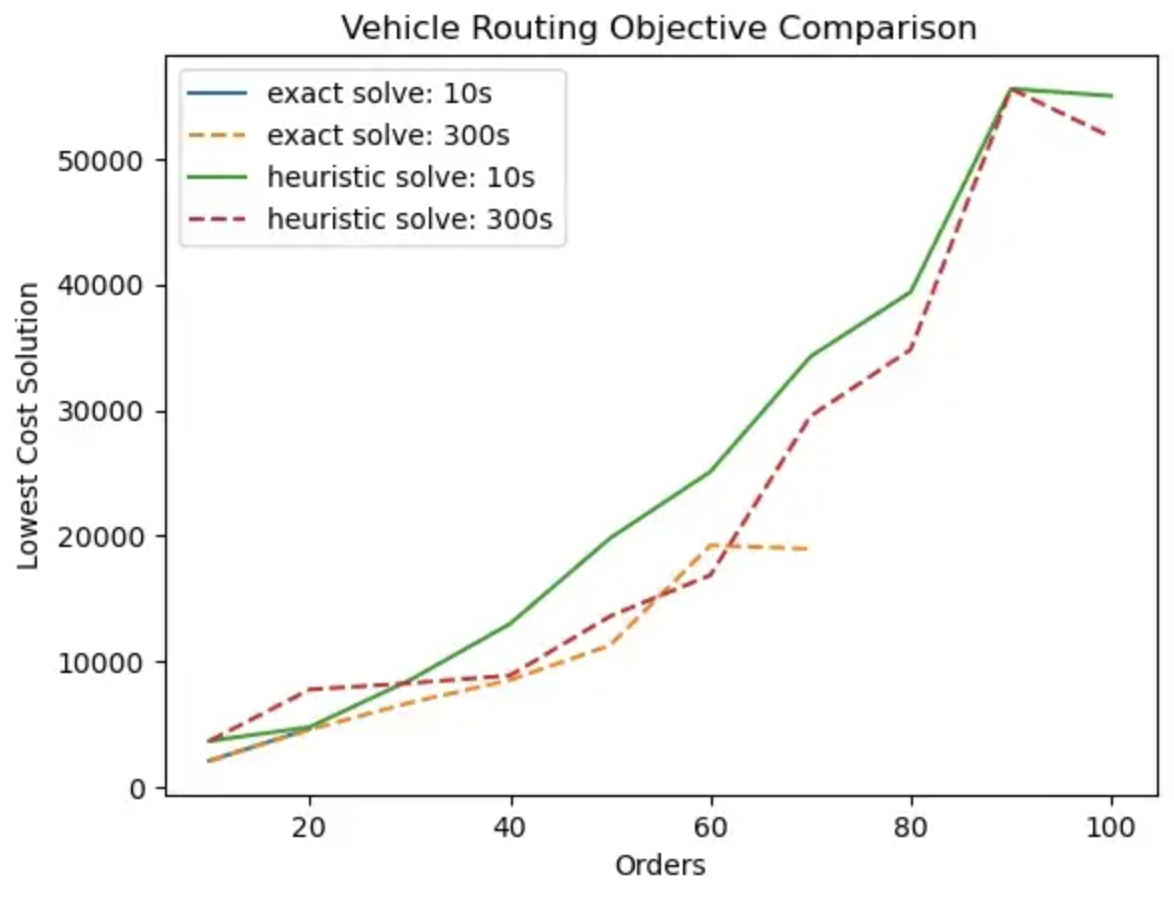
\includegraphics[]{col_gen_vs_direct.png}
					}
					\caption{Comparing the best found solutions at 10 seconds and 5 minutes for VRPs solved directly (exact) or with column generation (heuristic)}
					\label{p:compare}
				\end{figure}
			\end{column}
			\begin{column}{0.6\textwidth}
				\begin{itemize}
					\item Column generation heuristics can uncover solutions more quickly than direct solves.
					\item For example, consider the following:
					\begin{enumerate}[\bf a.]
						\item 10 seconds of column generation heuristic (green) \label{a}
						\item Five minutes of directly solving (orange) \label{b}
					\end{enumerate}
					\item Notice \textbf{\ref{a}.} regularly finds a solution that is 50\% as good as \textbf{\ref{b}.} but in 3\% time.
					\item \textbf{\ref{a}.} becomes advantageous past 70 orders when \textbf{\ref{b}.} can no longer find a solution.
				\end{itemize}
			\end{column}
		\end{columns}
		\vspace{-.5cm}
		\begin{block}{}
			Column generation heuristics can help us continue to find "good" solutions even problems become intractible to solve directly.
		\end{block}
		\normalsize
	\end{frame}

	\section{Vehicle Routing Problem Preliminaries}

	\begin{frame}[t]
		\frametitle{VRPTW Parameters, Variables, and Objective}
		\small
		\begin{itemize}
			\vspace{-.25cm}
			\item For simplicity, we will work with the VRP with Time Windows (VRPTW).
			\item The VRPTW has the following parameters:
			\begin{itemize}
				\item $c_{ij}$ covers cost to travel from node $i$ to node $j$.
				\item There are $n + 1$ nodes ($n$ customers and 1 depot (indexed 0)).
				\item There are $p$ vehicles.
				\item $[a_i, b_i]$ is the time window of customer $i$.
				\item $t_{ij}$ denotes the time to get from customer $i$ to customer $j$ (with service at customer $i$ included).
			\end{itemize}
			\item The VRPTW has the following variables:
			\begin{itemize}
				\item $s_i$ denotes the time that a vehicle starts serving customer $i$.
				\item $x_{ijk}$ has a value of 1 if the arc from node $i$ to node $j$ is in the optimal route driven by vehicle $k$ and 0 otherwise.
			\end{itemize}
			\item The VRPTW has the following objective:
			\begin{align*}
				\text{Min } \sum_{k = 1}^{p}{\sum_{i = 0}^{n}{\sum_{j = 0}^{n}{c_{ij}x_{ijk}}}}
			\end{align*}
		\end{itemize}
		\normalsize
	\end{frame}

	\begin{frame}[t]
		\frametitle{VRPTW Constraints}
		\footnotesize
		\vspace{-.25cm}
		The VRPTW has the following constraints:
		\begin{itemize}
			\item Each vehicle leaves each node that it enters:
			\begin{align}
				\sum_{i = 0}^{n}{x_{ijk}} = \sum_{i = 0}^{n}{x_{jik}} \qquad \forall j \in \{0,...,n\}, \enspace k \in \{1,...,p\} \label{c:leave_all}
			\end{align}
			\item Every node is entered once:
			\begin{align}
				\sum_{k = 1}^{p}{\sum_{i = 0}^{n}{x_{ijk}}} = 1  \qquad \forall j \in \{1,...,n\} \label{c:visit_all}
			\end{align}
			\item Every vehicle leaves the depot at most once:
			\begin{align}
				\sum_{j = 1}^{n}{x_{0jk}} \leq 1 \qquad \forall k \in \{1,...,p\} \label{c:leave_depot}
			\end{align}
		\end{itemize}
		\normalsize
	\end{frame}

	\begin{frame}[t]
		\frametitle{VRPTW Constraints}
		\footnotesize
		\vspace{-.25cm}
		\begin{itemize}
			\item Vehicle capacities are respected:
			\begin{align}
				\sum_{i = 0}^{n}{\sum_{j = 1}^{n}{q_{j} x_{ijk}}} \leq Q \qquad \forall k \in \{1,...,p\} \label{c:capacity}
			\end{align}
			\item Arrival happens after travel time is added to previous departure:
			\begin{align}
				s_i + t_{ij} - M * (1 - x_{ijk}) \leq s_j &\qquad \forall i \in \{0,...,n\}, \enspace j \in \{1,...,n\}, \enspace k \in \{1,...,p\} \qquad \label{c:travel_times} \\
				M = max \{b_i + t_{ij} - a_i\} &\qquad \forall i,j \in \{0,...,n\} \notag
			\end{align}
			\item The time window of each customer is respected:
			\begin{align}
				\qquad \qquad \qquad \qquad a_i \leq s_i \leq b_i \qquad \forall i \in \{0,...,n\} \qquad \qquad \qquad \qquad \qquad \label{c:time_windows}
			\end{align}
		\end{itemize}
		\vspace{.5cm}
		\begin{block}{}
			Since the VRPTW is intractible to solve directly for many production instances, reformulating can help us find something solvable.
		\end{block}
		\normalsize
	\end{frame}

	\begin{frame}[t]
		\frametitle{Example Solution}
		\small
		\vspace{-.25cm}
		From this formulation, if we were to plot the routes formed by the solution, we might see something like the following:
		\begin{figure}[h]
			\resizebox{.6\textwidth}{!}{%
				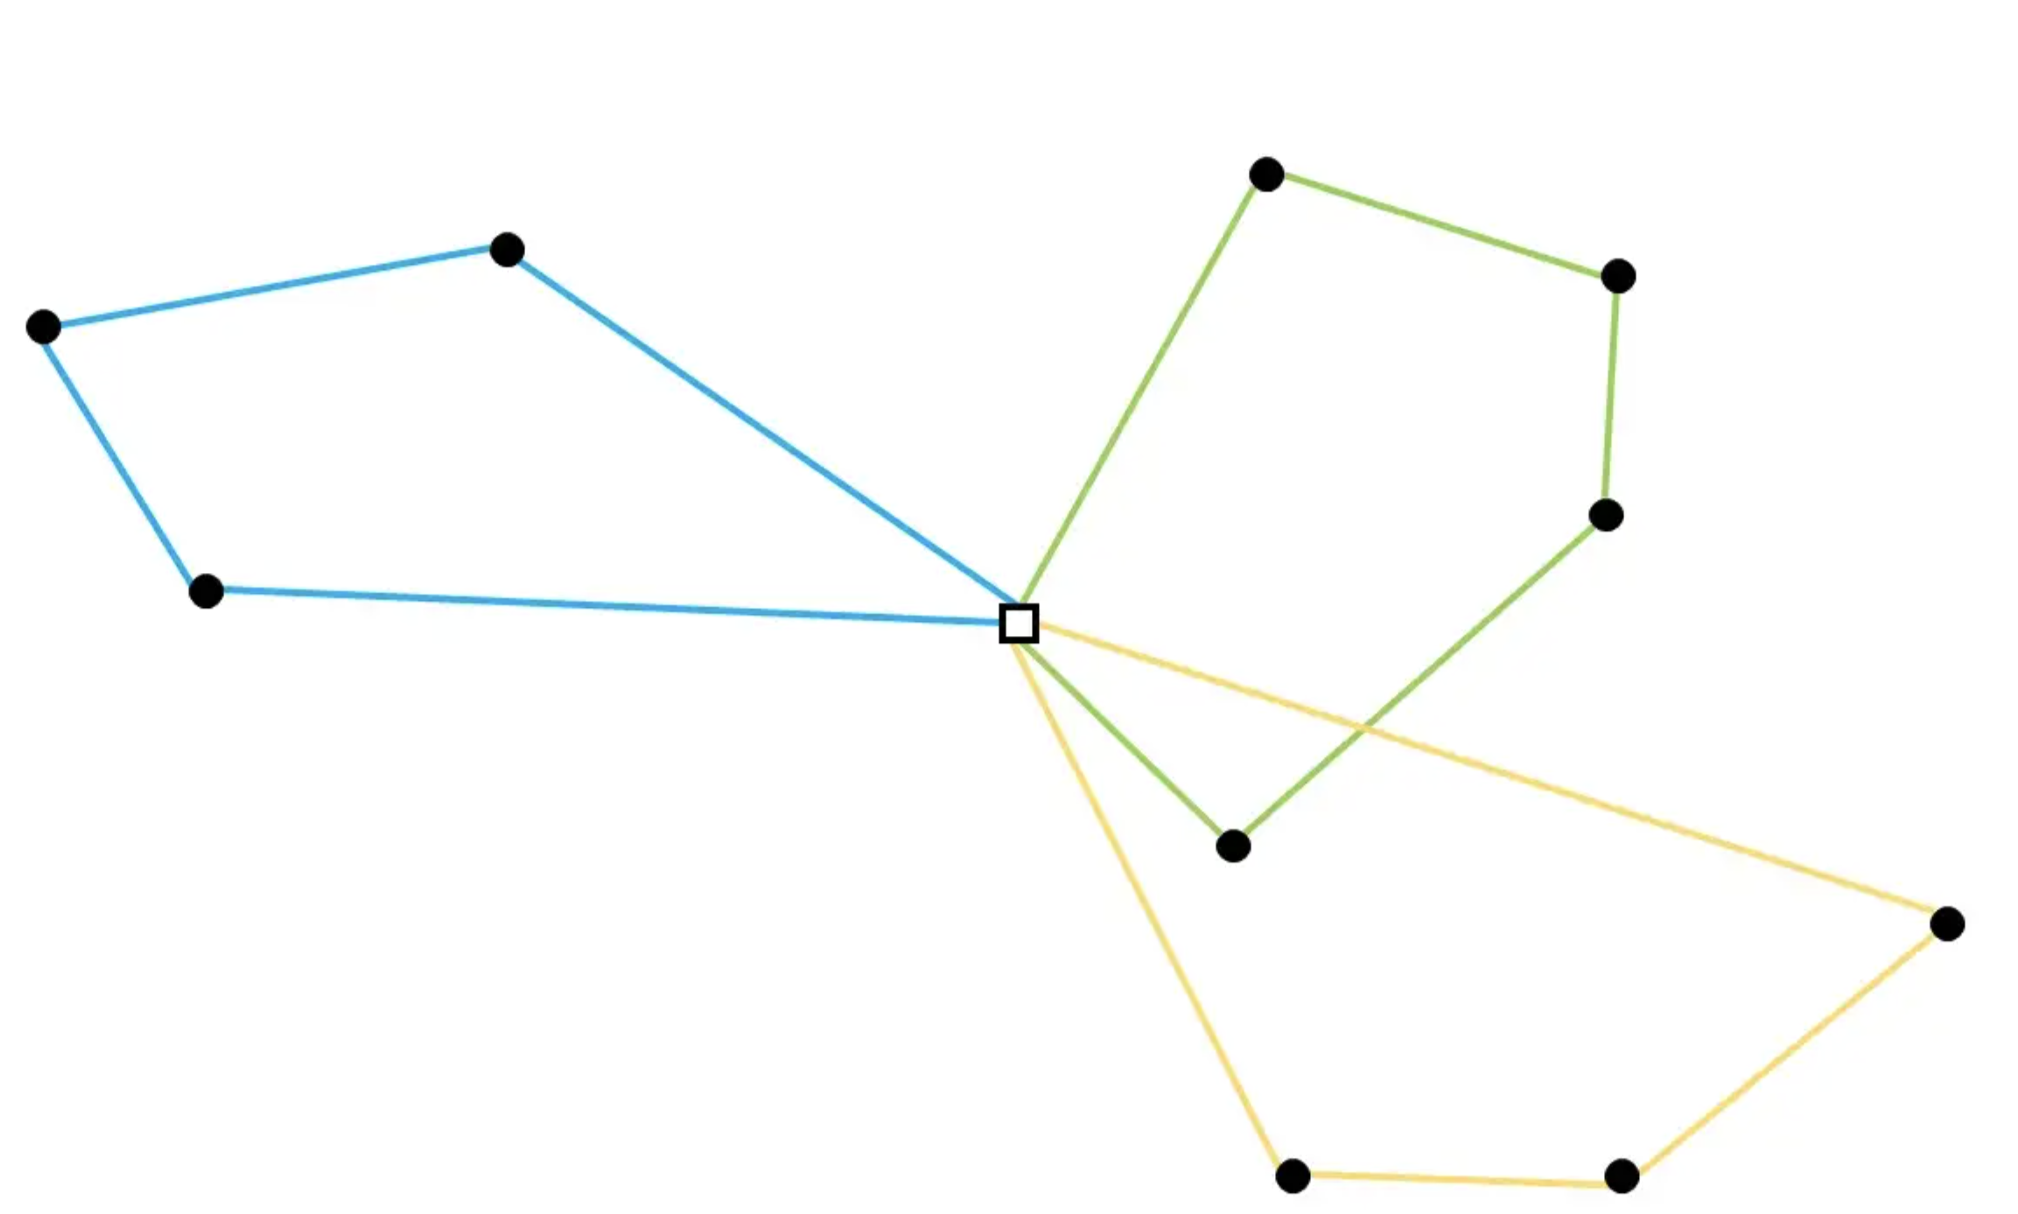
\includegraphics[]{solution.png}
			}
			\caption{A solution to a vehicle routing problem encodes each route with a distinct color and stop order by the edges between customers.}
			\label{p:solution}
		\end{figure}
		\normalsize
	\end{frame}

	\begin{frame}[t]
		\frametitle{Set Covering Problem (SCP) Reformulation}
		\footnotesize
		\begin{columns}[T]
			\begin{column}{0.55\textwidth}
				The SCP has the following parameters:
				\begin{itemize}
					\item $\Omega$ is the set of feasible vehicle routes.
					\item $c_k$ is the cost of route $r_k \in \Omega$.
					\item $a_{jk} = 1$ if route $r_k$ visits customer $j$ and 0 otherwise.
					\item $b_{ijk} = 1$ if route $r_k$ travels directly from customer $i$ to customer $j$ and 0 otherwise.
					\item Note the following relationships:
					\begin{align*}
						c_k &= \sum_{i=0}^n \sum_{j=0}^n c_{ij}b_{ijk} \\
						a_{jk} &= \sum_{i=0}^n b_{ijk}
					\end{align*}
				\end{itemize}
			\end{column}
			\begin{column}{0.45\textwidth}
				The SCP has the following variable:
				\begin{itemize}
					\item $z_k = 1$ if route $r_k$ is selected and 0 otherwise.
				\end{itemize}
				The SCP has the following objective:
				\begin{align*}
					\text{Min } \sum_{k \in \Omega}c_k z_k
				\end{align*}
				Subject to:
				\begin{align}
					\sum_{r_k \in \Omega} a_{jk} z_k \geq 1 \qquad \forall j \in \{1,...,n\} \label{c:set_covering}
				\end{align}
			\end{column}
		\end{columns}
		\vspace{0cm}
		\begin{block}{}
			The SCP is equivalent to the VRPTW, albeit often much larger. However, the SCP can be restricted to a much smaller problem while maintaining solution quality.
		\end{block}
		\normalsize
	\end{frame}

	\begin{frame}[t]
		\frametitle{Restricted Set Covering Problem (RSCP) Reformulation}
		\small
		\begin{columns}[T]
			\begin{column}{0.55\textwidth}
				The RSCP, w.r.t $\Omega' \subset \Omega $, (RSCP-$ \Omega' $) is formulated as follows:
				\begin{align}
					\text{Min } \sum_{k \in \Omega'}c_k z_k& \notag \\
					\text{s.t. } \sum_{r_k \in \Omega'} a_{jk} z_k \geq 1 &\qquad \forall j \in \{1,...,n\} \label{c:restricted_set_covering} \\
					z_k \in \{0, 1\} &\qquad \forall k \in \Omega' \notag
				\end{align}
			\end{column}
			\begin{column}{0.45\textwidth}
				The RSCP-$ \Omega' $ can efficiently approximate the VRPTW when:
				\begin{itemize}
					\item $ |\Omega'| $ is small.
					\item $ \Omega' $ covers all customers at low total cost.
				\end{itemize}
			\end{column}
		\end{columns}
		\vspace{2.75cm}
		\begin{block}{}
			We need to find a reasonable $ \Omega' $. For that, we will leverage column generation.
		\end{block}
		\normalsize
	\end{frame}

	\section{Column Generation Preliminaries}
	
	\begin{frame}[t]
		\frametitle{A Column Generation Heuristic for the VRPTW}
		\small
		\vspace{-.25cm}
		Our column generation heuristic can be broken down as follows:
		\begin{itemize}
			\item Initialize
			\begin{itemize}
				\item Find an initial set of feasible covering routes, $ \Omega'_0 $, which could be:
				\begin{itemize}
					\item The set of singleton routes.
					\item The K nearest neighbors for each customer.
				\end{itemize}
			\end{itemize}
			\item Iterate (let $ i $ be the iteration index)
			\begin{itemize}
				\item Solve the LP relaxation of RSCP-$ \Omega'_i $.
				\item Find $ \Gamma_i \subset \Omega \setminus \Omega'_i $, a set of improving routes for the RSCP-$ \Omega'_i $.
				\item Let $ \Omega'_{i+1} = \Omega'_i \cup \Gamma_i $.
				\item Increment $ i $ and repeat the above until $ \Gamma_i = \emptyset $ or we are satisfied.
			\end{itemize}
			\item Cover
			\begin{itemize}
				\item Solve the final RSCP-$ \Omega_i $.
				\item Return the chosen routes.
			\end{itemize}
		\end{itemize}
		\vspace{-.25cm}
		\begin{block}{}
			We can determine if a route improves the solution for the RSCP-$ \Omega_i $ by calculating its reduced cost.
		\end{block}
		\normalsize
	\end{frame}

	\begin{frame}[t]
		\frametitle{Dual LP Relaxation for the SCP}
		\small
		\begin{columns}[T]
			\begin{column}{0.6\textwidth}
				Parameters:
				\begin{itemize}
					\item Let $ A $ represent the matrix of $ a_{jk} $.
					\item $ A_k = [a_{1k}, ..., a_{nk}]^T $, i.e. stops of route $ r_k $.
					\item $ c $ is vector of route costs $ [c_1, ..., c_{|\Omega|}]^T $.
				\end{itemize}
				Sets:
				\begin{itemize}
					\item $ B $ is the indices of basis variables for the solution to the RSCP-$ \Omega_i $ LP relaxation.
					\item $ N $ is remaining variable indices in the SCP.
				\end{itemize}
			\end{column}
			\begin{column}{0.4\textwidth}
				Variables:
				\begin{itemize}
					\item $ y $ is row reduced costs.
					\item $ s $ is column reduced costs.
				\end{itemize}
				Formulation:
				\begin{align*}
					\text{Max } 1^T &y  \\
					\text{s.t. } A^T &y + s = c \\
					&y, s \geq 0
				\end{align*}
			\end{column}
		\end{columns}
		\vspace{0cm}
		\begin{block}{}
			From Linear Programming (LP) theory, we can conclude the following about the SCP solution with basis $ B $:
			\begin{itemize}
				\item The reduced cost of $ z_k $ (a.k.a. $ s_k $) is $ c_k - A^T_k y $ for all $ k \in N $.
				\item If $ c_k - A^T_k y < 0 $, then adding $ r_k $ to RSCP-$ \Omega_i $ will improve its objective.
			\end{itemize}
		\end{block}
		\normalsize
	\end{frame}

	\begin{frame}[t]
		\frametitle{A Critical Observation}
		\small
		\begin{itemize}
			\item We can evaluate the reduced costs of routes not in the RSCP with the dual solution to the SCP.
			\item Done explicitly, this creates the size of problem we're trying to avoid.
			\item However, we can do so implicity by solving the Pricing Problem, which includes the following:
			\begin{itemize}
				\item Minimize the reduced costs of a route.
				\item Subject routes to feasibility defined in the VRPTW.
				\item Return routes found during the optimization problem with negative costs.
			\end{itemize}
		\end{itemize}
		\normalsize
	\end{frame}

	\section{Pricing Feasible Routes for the VRPTW}
	
	\begin{frame}[t]
		\frametitle{Connecting Previous Formulations to the Pricing Problem}
		\small
		\begin{columns}[T]
			\begin{column}{0.6\textwidth}
				By the definition of $b_{ijk}$
				\begin{align*}
					b_{ijk} = x_{ijk} \qquad \forall i, j \in \{0, ..., n\}, \; k \in \Omega
				\end{align*}		
				By the definition of $a_{jk}$
				\begin{align*}
					a_{jk} = \sum_{i=0}^n x_{ijk} \qquad \forall j \in \{0, ..., n\}, \; k \in \Omega
				\end{align*}		
				Then, reduced costs can be rewitten as
				\begin{align*}
					c_k - A_k^T y = {\sum_{i = 0}^{n}{\sum_{j = 0}^{n}{c_{ij}x_{ijk}}}} - {\sum_{j = 1}^{n} \Bigg( y_j \sum_{i = 0}^{n} x_{ijk} \Bigg)}
				\end{align*}
			\end{column}
			\begin{column}{0.4\textwidth}
				The Pricing Problem differs from the VRPTW in the following ways:
				\begin{itemize}
					\item Index $k$ is removed from arc variables, $x$, since we solve for a single route.
					\item Constraint 2 is removed since it is accounted for in the (R)SCP.
					\item The objective is to minimize the \textbf{reduced} cost of the route.
				\end{itemize}
			\end{column}
		\end{columns}
		\vspace{.25cm}
		\begin{block}{}
			Consequently, the Pricing Problem is a factor of $ \frac{1}{k} $ as large as the original VRPTW, which is why our column generation heuristic is tractible.
		\end{block}
		\normalsize
	\end{frame}

	\begin{frame}[t]
		\frametitle{Pricing Problem Formulation}
		\small
		\vspace{-.25cm}
		We seek to minimize the reduced cost of a given route:
		\begin{align*}
			\text{Min } \sum_{i = 0}^{n}{\sum_{j = 0}^{n}{c_{ij}x_{ij}}} - \sum_{j = 1}^{n} \Bigg( y_j \sum_{i = 0}^{n} x_{ij} \Bigg)
		\end{align*}
		Subject to:
		\begin{itemize}
			\item The route leaves each node that it enters:
			\begin{align}
				\sum_{i = 0}^{n}{x_{ij}} = \sum_{i = 0}^{n}{x_{ji}} \qquad \forall j \in \{0,...,n\} \label{c:leave_customer_pricing}
			\end{align}
			\item The route leaves the depot at most once:
			\begin{align}
				\sum_{j = 1}^{n}{x_{0j}} \leq 1 \label{c:leave_depot_pricing}
			\end{align}
		\end{itemize}
		\normalsize
	\end{frame}

	\begin{frame}[t]
		\frametitle{Pricing Problem Formulation}
		\small
		\vspace{-.25cm}
		\begin{itemize}
			\item The route respects vehicle capacity:
			\begin{align}
				\sum_{i = 0}^{n}{\sum_{j = 1}^{n}{q_{j} x_{ij}}} \leq Q \label{c:capacity_pricing}
			\end{align}
			\item Arrival happens after travel time is added to previous departure:
			\begin{align}
				s_i + t_{ij} - M * (1 - x_{ij}) \leq s_j \qquad \forall i \in \{0,...,n\}, \enspace j \in \{1,...,n\} \label{c:travel_times_pricing}
			\end{align}
			\item The route respects the time window of each customer:
			\begin{align}
				a_i \leq s_i \leq b_i \qquad \forall i \in \{0,...,n\} \label{c:time_window_pricing}
			\end{align}
		\end{itemize}
		\vspace{.5cm}
		\begin{block}{}
			By collecting all negative solutions found while solving the Pricing Problem, we generate a set of routes improving the RSCP-$ \Omega_i $.
		\end{block}
		\normalsize
	\end{frame}

	\begin{frame}[t]
		\frametitle{Why Formulate the Pricing Problem as a MIP?}
		\small
		\vspace{-.25cm}
		Pricing problems are often formulated as Dynamic Progams (DPs). In practice, I've seen MIP formulations implemented instead for the following reasons:
		\begin{itemize}
			\item Clients have diverse constraints in their pricing problems, necessitating rich modeling capabilities.
			\item MIPs often find many solutions (i.e. routes) in a single solve.
			\item MIPs can be resolved with slight adjustments to the constraints, generating additional routes.
			\item Each MIP solve can possibly be warm started.
		\end{itemize}
		\normalsize
	\end{frame}

	\section{Column Generation Closing Thoughts}

	\begin{frame}[t]
		\frametitle{Recap: A Column Generation Heuristic for the VRPTW}
		\small
		\vspace{-.25cm}
		Our column generation heuristic can be broken down as follows:
		\begin{itemize}
			\item Initialize.
			\begin{itemize}
				\item Find an initial set of feasible covering routes, $ \Omega'_0 $, which could be:
				\begin{itemize}
					\item The set of singleton routes.
					\item The K nearest neighbors for each customer.
				\end{itemize}
			\end{itemize}
			\item Iterate (let $ i $ be the iteration index).
			\begin{itemize}
				\item Solve the LP relaxation of RSCP-$ \Omega'_i $.
				\item Find $ \Gamma_i \subset \Omega \setminus \Omega'_i $, a set of improving routes for the RSCP-$ \Omega'_i $ \textbf{by solving the Pricing Problem}.
				\item Let $ \Omega'_{i+1} = \Omega'_i \cup \Gamma_i $.
				\item Increment $ i $ and repeat the above until $ \Gamma_i = \emptyset $ or we are satisfied.
			\end{itemize}
			\item Cover.
			\begin{itemize}
				\item Solve the final RSCP-$ \Omega_i $.
				\item Return the chosen routes.
			\end{itemize}
		\end{itemize}
		\normalsize
	\end{frame}

	\begin{frame}[t]
		\frametitle{A Note on Branch-and-Price}
		\small
		\vspace{-.25cm}
		\begin{block}{}
			Our column generation heuristic is unlikely to yield an optimal solution to the VRPTW. Branch-and-Price is often used if one is desired.
		\end{block}
		\vspace{-.25cm}
		\begin{itemize}
			\item Branch-and-Price retains tractibility by solving RSCP LP relaxations and Pricing Problems.
			\item It differs from our column generation heuristic as follows:
			\begin{itemize}
				\item If the LP relaxation solution to the final RSCP-$ \Omega_i $ is not integer feasible, branching occurs, and our algorithm repeats on each branch.
				\item One branch requires all new routes to visit a location $ j $ immediately after location $ i $ (i.e. $ x_{ijk} = 1 $).
				\item The other branch prohibits all new routes from visiting a location $ j $ immediately after location $ i $ (i.e. $ x_{ijk} = 0 $).
			\end{itemize}
			\item Consequently, Branch-and-Price takes longer to run and implement.
			\item Dominique Feillet's “A Tutorial on Column Generation and Branch-and-Price for Vehicle Routing Problems” provides further details.
		\end{itemize}
		\normalsize
	\end{frame}

	\section{Implementation Details}
	
	\begin{frame}[t]
		\frametitle{Important Parameters}
		\small
		\vspace{-.25cm}
		The following are paramaters input to our column generation algorithm:
		\vspace{.25cm}
		\begin{table}[ht]
			\centering
			\begin{tabular}{|p{0.4\linewidth}|p{0.4\linewidth}|}
				\hline
				\textbf{Parameter} & \textbf{Trade-Off} \\ 
				\hline
				Solutions per Pricing Problem solve & RSCP solve time vs. Pricing Problem solves \\ 
				\hline
				Pricing Problem MIP gap & quantity vs. quality of columns generated \\ 
				\hline
				Pricing Problem time limit & quantity vs. quality of columns generated \\ 
				\hline
				Relative RSCP LP resolve improvement & solution quality vs. solve time \\ 
				\hline
				Ratio of time iterating vs. covering & number of routes found vs. quality of routes chosen \\ 
				\hline
			\end{tabular}
		\end{table}
		\vspace{.25cm}
		\begin{block}{}
			The values of the following parameters can vastly change solve time and solution quality. Practitioners should tune each to ensure desired results.
		\end{block}
		\normalsize
	\end{frame}

	\begin{frame}[t]
		\frametitle{Important GurobiPy API Endpoints}
		\small
		\vspace{-.25cm}
		The following "out of the ordinary" GurobiPy API Endpoints were used in the implementation:
		\vspace{.25cm}
		\begin{table}[ht]
			\centering
			\begin{tabular}{|p{0.3\linewidth}|p{0.5\linewidth}|}
				\hline
				\textbf{Endpoint} & \textbf{Meaning} \\ 
				\hline
				Constraint.pi & Row reduced costs \\ 
				\hline
				PoolSolutions & Max number of solutions to cache \\ 
				\hline
				Model.SolCount & Number of solutions cached \\ 
				\hline
				Model.SolutionNumber & Index of the current solution \\ 
				\hline
				Model.PoolObjVal & Objective value of the current solution \\
				\hline
				Column() & Object that sets nonzero constraint coefficients for new variables \\ 
				\hline
			\end{tabular}
		\end{table}
		\vspace{1cm}
		\begin{block}{}
			For practitioners seeking to use a different MIP solver, one will want its API to include attributes similar to the above.
		\end{block}
		\normalsize
	\end{frame}

	\begin{frame}[t]
		\frametitle{GitHub Repo}
		\small
		Source code for the implementation of our column generation heuristic can be found on \textcolor{blue}{\href{https://github.com/spkelle2/vehicle_routing_column_generation}{GitHub}} (spkelle2/vehicle\_routing\_column\_generation).
		\normalsize
	\end{frame}

	\section{Questions}
		
\end{document}
